
\xpartbox{Face Matching}

\begin{xpsectionbox}{Description}{}

Localized face/profile regions  need to be matched against a query face/profile picture, which may come from an existing (and possibly annotated) image, or from a new photograph, that face matcher has not seen before. Hence the face matching method needs to be approximate to accommodate wide variations in the appearance, yet it needs to be fairly exact to eliminate numerous false positive hits.

%\begin{minipage}{0.4\linewidth}
%
%\begin{itemize}
%	  \item low-level image features (Haar, LBP, etc.)
%	  \item high-level facial landmarks (eye(s), nose, mouth, ear(s), chin, etc.)
%	  \item skin color
%\end{itemize}
%\end{minipage}
%\begin{minipage}{0.6\linewidth}
%
%\begin{center}
%%			%\hspace{-5cm}
%%			\vspace{-1cm}
%			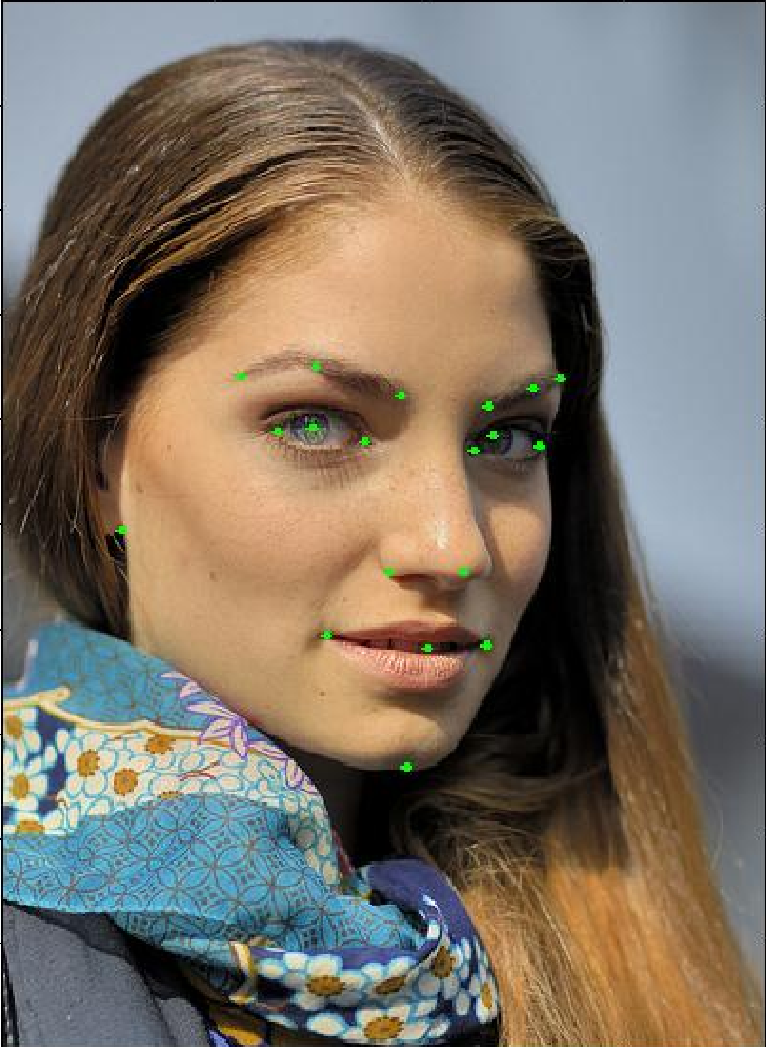
\includegraphics[height=0.25\linewidth]{images/facial_landmarks}
%			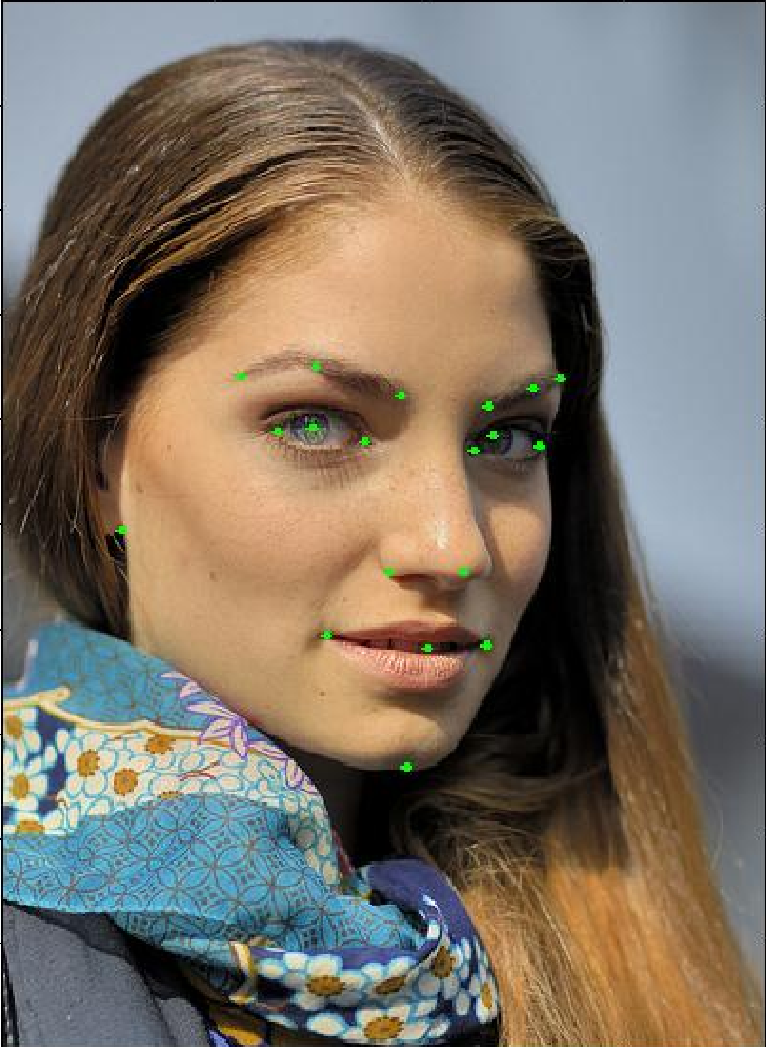
\includegraphics[height=0.25\linewidth]{images/facial_landmarks}
%\end{center}
%
%\end{minipage}
\end{xpsectionbox}

%\begin{xpsectionbox}{Challenges}{}
%
%\begin{minipage}{0.4\linewidth}
%\begin{itemize}
%	  \item local descriptors (Haar, SIFT, SURF, ORB)
%	  \item low-quality images
%	  \item various lighting conditions
%	  \item frontal vs. profile faces
%	  \item occlusions, facial hair, spectacles, hat, etc.
%\end{itemize}
%\end{minipage}
%\begin{minipage}{0.6\linewidth}
%\begin{center}
%			\vspace{-2cm}
%			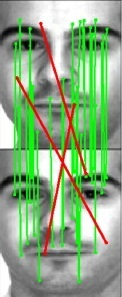
\includegraphics[height=0.45\linewidth]{images/face_match_sift}
%\end{center}
%\end{minipage}
%
%\end{xpsectionbox}

\xpartbox{Solution}

%--------------------------------------------------------------------------------------------------------------------
\begin{xpsectionbox}{}{}


\begin{minipage}{0.5\linewidth}

{\vspace*{0.2cm}\noindent\hspace*{0.2cm}{\bf\Titlesize Method}\newline}{\vspace{-0.75cm}}

\begin{itemize}
	  \item Haar/SIFT/SURF/ORB
	  \item rotation invariant metrics
	  \item ...
\end{itemize}
\begin{center}
			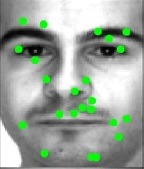
\includegraphics[height=0.25\linewidth]{images/face_sift}
\end{center}

%\bf{Drawbacks:}
%\begin{itemize}
%	  \item small size faces not detectable
%	  \item lighting/occlusion deteriorates results 
%\end{itemize}
%\begin{center}
%			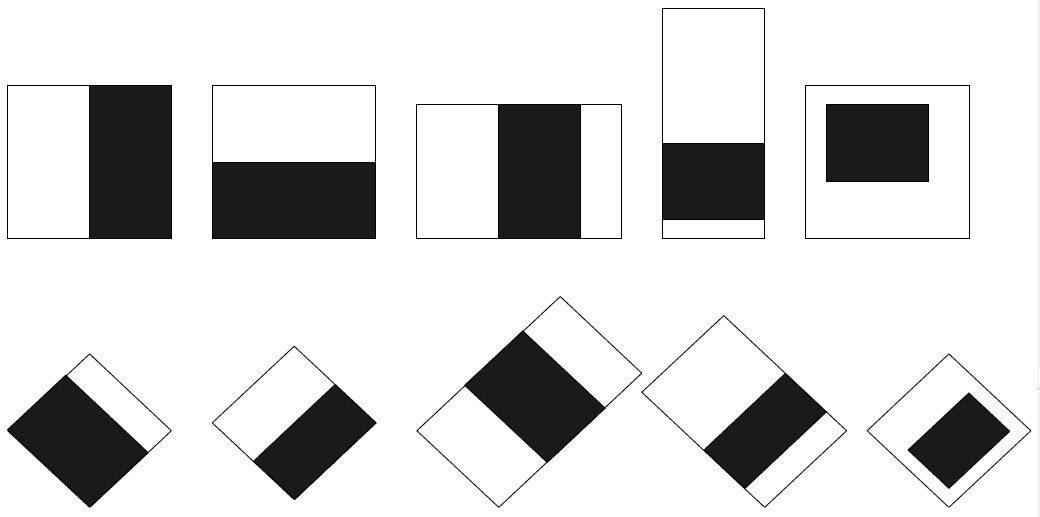
\includegraphics[height=0.25\linewidth]{images/Haar_features}
%\end{center}

\end{minipage}
\begin{minipage}{0.5\linewidth}

{\vspace*{0.2cm}\noindent\hspace*{0.2cm}{\bf\Titlesize Improvements}\newline}{\vspace{-0.75cm}}

\begin{itemize}
	  \item re-ranking based on
	  	\begin{itemize}
	  		\item Borda count
	  		\item weighted Borda count
	  		\item distances
	  	\end{itemize}
	  \item fast indexing (tree structure)
	  \item ...
\end{itemize}
\begin{center}
			%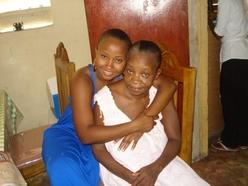
\includegraphics[height=0.2\linewidth]{images/Lena_RGB}
			%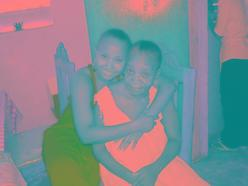
\includegraphics[height=0.2\linewidth]{images/Lena_LAB}
			%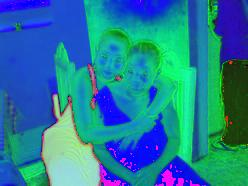
\includegraphics[height=0.2\linewidth]{images/Lena_HSV}
			%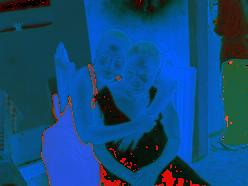
\includegraphics[height=0.2\linewidth]{images/Lena_LUV}
\end{center}
%\bf{Advantages:}
%\begin{itemize}
%	  \item high precision skin detection(91\%)  
%	  \item skin maps focus the face finding
%	  \item enhance skin region intensities
%\end{itemize}
%\begin{center}
%			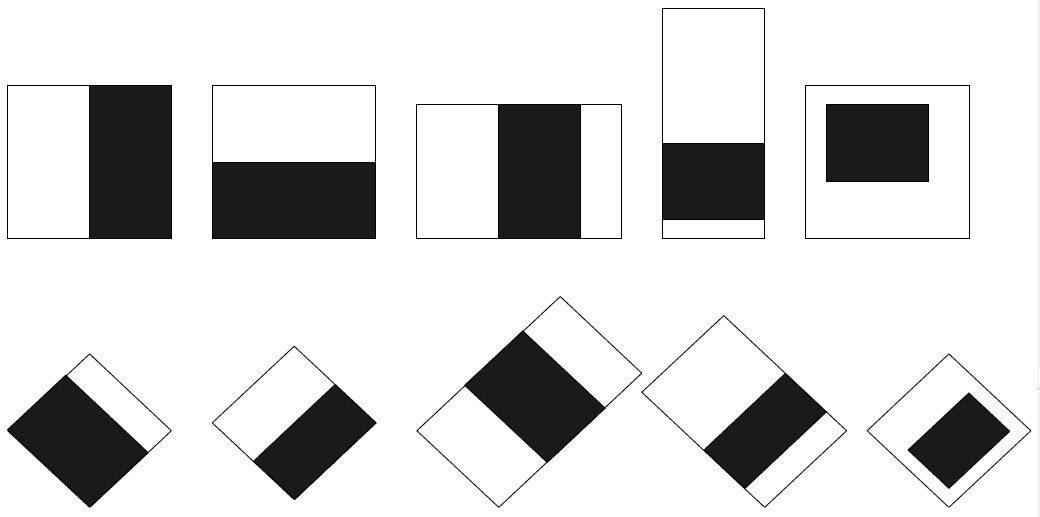
\includegraphics[height=0.2\linewidth]{images/Haar_features}
%\end{center}
\end{minipage}
\end{xpsectionbox}

\xpartbox{Experiments}

\begin{xpsectionbox}{}{}
Our experiments with the annotated HEPL-4K images, and on HEPL-62mod (372 = 62 images with 6 synthetic modifications, e.g. crop, scale and rotate). Accuracy (F-score) figures are reported in the table.

\begin{tabular*}{0.75\textwidth}{@{\extracolsep{\fill}} | c | c | c | c | c | }
  \hline
  dataset & HAAR & SIFT & SURF & ORB \\
  \hline
  HEPL-4K & {\bf0.99} & 0.98 & 0.96 & 0.95 \\
  \hline
  HEPL-62mod  & 0.44  & {\bf0.81}  & 0.52 & 0.56 \\
  \hline
\end{tabular*}

We have also experimented with combining the descriptor match distances by using a generalized geometric mean, and found that a combination of HAAR*ORB*SIFT*SURF produce a better F score (by about 5 percentage points), than either of them. Inclusion of a weak descriptor may hurt the ensemble.
\end{xpsectionbox}

%\xpartbox{Automatic Bangla Recognition}
%
%%--------------------------------------------------------------------------------------------------------------------
%\begin{xpsectionbox}{Motivation}{}
%
%With the availability of electronic tablets at a cost affordable to common Indians, online handwriting recognition for Indian scripts has gained importance.
%
%\begin{minipage}{0.6\linewidth}
%
%\vspace{1cm}
%{\bf Existing problems:}
%
%\begin{itemize}
%	  \item no unconstrained online Indian script recognizer  
%	  \item large symbol set for Bangla
%	  \item no reliable segmentation strategy for Bangla
%\end{itemize}
%
%
%{\bf General solutions:}
%
%\begin{itemize}
%	  \item analytical (segmentation based on pseudo-characters, graphemes), etc. followed by classification   
%	  \item holistic (no segmentation, limited to small vocabulary)
%	  \item HMM based (segmentation and recognition integrated in the model)
%\end{itemize}
%
%{\bf Proposed approach:  Combination of ...}
%
%\begin{itemize}
%	  \item sub-stroke level feature representation
%	  \item HMM based model for cursively written words
%	  \item context dependent sub-word units
%\end{itemize}
%
%\end{minipage}
%\begin{minipage}{0.4\linewidth}
%\begin{center}
%		\vspace{-1cm}
%		\hspace{1cm}
%		\center
%		%\includegraphics[width=0.95\linewidth]{images/input-using-handwriting-recognition.jpg}
%		%\includegraphics[width=0.99\linewidth]{images/tablet.jpg}
%		%\includegraphics[width=0.95\linewidth]{images/hp_tablet.jpg}
%		Wacom Intuos2
%		%\includegraphics[width=0.95\linewidth]{images/Wacom-Intuos2.jpg}
%		\end{center}
%
%\end{minipage}
%
%\end{xpsectionbox}
%%--------------------------------------------------------------------------------------------------------------------
%
%\xpartbox{Preprocessing}
%
%%--------------------------------------------------------------------------------------------------------------------
%\begin{xpsectionbox}{Preprocessing and Sub-Stroke Segmentation}{}
%
%\begin{minipage}{0.5\linewidth}
%
%{\bf Preprocessing:}
%
%\begin{itemize}
%	  \item size normalization (100, original aspect ratio)   
%	  \item smoothing (moving average)
%	  \item re-sampling (distance between two points is $7.0$)
%\end{itemize}
%\end{minipage}
%\begin{minipage}{0.5\linewidth}
%
%
%\vspace{-1.3cm}
%{\bf Stroke segmentation:}
%
%
%\begin{itemize}
%	  \item each stroke is divided in sub-strokes  
%	  \item each sub-stroke with length less than $5$ is discarded
%\end{itemize}
%\end{minipage}
%
%\begin{center}
%		%\vspace{-3cm}
%		%\hspace{1cm}
%		%\center
%		%\includegraphics[width=0.5\linewidth]{images/Aassam-SubStrokes-Numbered.pdf}
%		
%		%\includegraphics[width=0.85\linewidth]{images/unbalanced.pdf}
%\end{center}
%
%{\bf Algorithm:}
%
%\vspace{0.5cm}
%
%\noindent \(P_0, P_1, P_2, \ldots, P_N\) sequence of points from a stroke
%
%\noindent STEP 1: \(i = 0;\) \(j = 1;\)
%
%\noindent STEP 2: Compute \(\theta = \mbox{angle}(P_i,P_j);\)
%
%\noindent STEP 3: {\bf If} \((j < N+1)\)
%
%\hspace{2cm} Compute \(\alpha_j\) = angle \((P_i,P_j);\) %and
%
%\hspace{2cm} \(\beta_j\) = angle \((P_{j-1}, P_j);\)
%
%\hspace{1.2cm} {\bf else}
%
%\hspace{2cm} go to STEP 6
%
%\noindent STEP 4: \hspace{-0.3cm}{\bf If} $(\min\{|\theta-\alpha_j|,360^\circ-|\theta-\alpha_j|\} < 90^\circ \mbox{ and }\min\{|\beta_{j-1}-\beta_j|, 360^\circ-|\beta_{j-1}-\beta_j|\} < 90^\circ)$
%
%\hspace{2cm} \(j = j + 1;\)
%
%\hspace{2cm} GOTO STEP 3
%
%\noindent STEP 5: Segment the stroke at \(P_{j-1}\)
%
%\hspace{1.2cm} \(i = j;\) \(j = j + 1;\)
%
%\hspace{1.2cm} GOTO STEP 2
%
%\noindent STEP 6: STOP
%
%
%\end{xpsectionbox}
%%--------------------------------------------------------------------------------------------------------------------
%
%\xpartbox{Feature Extraction}
%
%%--------------------------------------------------------------------------------------------------------------------
%\begin{xpsectionbox}{Feature Extraction}{}
%
%\begin{minipage}{0.6\linewidth}
%{\bf Steps:}
%
%\begin{itemize}
%	  \item each sub-stroke $S$ is represented by polylines   
%	  \item find six equidistant points \(Q_0,Q_1,\ldots,Q_5\) on $S$
%	  \item calculate the angle $\theta_i$ between x-axis and $Q_{i-1}Q_i$\\ $(i=1,2,\ldots,5;$ $0^\circ \le \theta_i < 360^\circ)$
%		\item normalized gravity center ($\overline{X},\overline{Y})$ of $S$ with respect to\\height ($100$) and width ($W$)
%		\item $l$ is the total length of the sub-stroke $S$
%\end{itemize}
%
%{\bf Result:}
%
%\begin{itemize}
%	  
%		\item 8-dimensional feature vector (\(F=(\theta_1,\ldots,\theta_5,\overline{X},\overline{Y},l)\))
%\end{itemize}
%\end{minipage}
%\begin{minipage}{0.4\linewidth}
%\center
%%\includegraphics[width=0.99\linewidth]{images/sixEquidistantPoints.pdf}
%\end{minipage}
%
%\end{xpsectionbox}
%%--------------------------------------------------------------------------------------------------------------------
%%--------------------------------------------------------------------------------------------------------------------
%
%\xpartbox{Modeling}
%
%\begin{xpsectionbox}{Writing Model}{}
%
%\begin{minipage}{0.6\linewidth}
%
%%\vspace{1cm}
%{\bf Advantages of the modeling:}
%
%\begin{itemize}
%	  \item segmentation/recognition based on HMM 
%	  \item word are constructed from characters
%	  \item complex and robust parameter estimation
%\end{itemize}
%
%\vspace{1cm}
%
%{\bf Challenges in Bangla word modeling:}
%
%\begin{itemize}
%	  \item the notion of basic unit in Bangla is not obvious 
%	  \item basic characters and shape modifiers
%	  \item basic character$+$shape modifiers $=$ new characters
%	  \item characters merged $=$ compound characters
%	  \item potentially huge number of basic modeling units
%\end{itemize}
%
%\vspace{1cm}
%
%{\bf Context-dependent sub-word units for Bangla:}
%
%\begin{itemize}
%	  \item inspired by triphone units from speech recognition
%	  \item Baseline: fully decomposed model (including split up complex modifiers)
%	  \item models include one symbol of left and right context $\Rightarrow$ large number of potential units
%	  \item apply greedy clustering to state-space of intermediate model in order to determine to-be-shared model parameters in purely data-driven manner 
%\end{itemize}
%
%
%\end{minipage}
%\begin{minipage}{0.4\linewidth}
%\begin{center}
%		\vspace{-13cm}
%		\hspace{1cm}
%		\center
%		
%		Basic Bangla characters
%		%\includegraphics[width=0.99\linewidth]{images/BasicCharacter-ICFHR.pdf}
%		
%		
%		\vspace{1cm}
%		Compound Bangla characters
%		%\includegraphics[width=0.99\linewidth]{images/CompoundChar-ICFHR.pdf}
%		\end{center}
%
%\end{minipage}
%
%\vspace{1cm}
%
%\center
%Vowel (left) and consonant (right) modifiers
%%\includegraphics[width=0.99\linewidth]{images/Modifier-ICFHR.pdf}
%
%\end{xpsectionbox}
%--------------------------------------------------------------------------------------------------------------------

%--------------------------------------------------------------------------------------------------------------------